\documentclass[11pt]{article}
\usepackage{fullpage}
\usepackage{amsmath}
\usepackage{amssymb}
\usepackage{gensymb}
\usepackage{graphicx}
\usepackage{cancel}
\usepackage{hyperref}
\usepackage{tikz}
\usepackage{verbatim}
\usepackage{listings}
\usepackage{forest}
\hypersetup{
    colorlinks,
    citecolor=black,
    filecolor=black,
    linkcolor=blue,
    urlcolor=black
}

\lstset{language=C++,
    basicstyle=\ttfamily,
    keywordstyle=\color{blue}\ttfamily,
    stringstyle=\color{red}\ttfamily,
    commentstyle=\color{gray}\ttfamily,
    morecomment=[l][\color{magenta}]{\#}
}

\usetikzlibrary{calc, shapes.geometric, arrows}

\tikzstyle{redrect} = [rectangle, rounded corners, minimum width=3cm, 
    minimum height=1cm,text centered, draw=black, fill=red!30]
    
\tikzstyle{bluerect} = [rectangle, rounded corners, minimum width=3cm, 
    minimum height=1cm,text centered, draw=black, fill=blue!30]

\tikzstyle{orangerect} = [rectangle, rounded corners, minimum width=3cm, 
    minimum height=1cm,text centered, draw=black, fill=orange!30]

\tikzstyle{arrow} = [thick,->,>=stealth]


\title{\vspace{10em}ME 759 Final Project Report \\ Default Project 1: Distributed Task Library}
\author{William Jen \\ University of Wisconsin-Madison}
\date{December 2017}

\begin{document}
    \maketitle

    \pagebreak
    \section{Abstract}
    
    \pagebreak
    \tableofcontents
    \pagebreak
    
    \section{Introduction}
        Default Project 1 was described as an "OpenMP-based parallel and decoupled mechanism for
        asynchronous update of an on-going process.". In other words, a parent job $P$ may run in 
        a loop. Within that loop, it may spawn children tasks $C_1 \ldots C_n$ that can be run on either
        the same machine in a different thread or a separate machine entirely. Furthermore, these tasks may
        use GPU acceleration, so if a child task is set to run on a different machine, it must be run on a 
        machine with a GPU. Additionally, the parent task $P$ must not advance to the next iteration of the loop
        before all of its children tasks have completed. The goal of this project is to define a software framework 
        that will allow the programmer to spawn child tasks on the location of their choice (same host, new host, 
        GPU-enabled host) with the ability to wait for children tasks.
    
    \section{Design}
        The Distributed Task Library breaks this project into two parts: task running on the local machine and 
        task running on remote machines. To maximize portability, cross-platform libraries and technologies 
        were selected, such as C++11 threads, OpenMPI, and Google Protobuf. The main idea behind this library
        was to allow the programmer to specify function pointers to their code, and have the library take care of
        the rest. 

        \subsection{Creating Jobs Locally}
            \subsubsection{A Simple Example}
                Creating jobs locally is very similar in concept to OpenMP tasks without macros. In other words,
                the user can spawn a task, and that task can spawn children tasks. Before the parent can complete,
                it must wait for its children to finish. 
                
                The Task class is responsible for creating and running local jobs and works by spinning off
                a thread for each job. This class is best explained via an example.
                
                \pagebreak
                
                \begin{lstlisting}[language=C++]
#include <iostream>
#include "Task.hpp"

void jobB(std::shared_ptr<dtl::Task> parent) 
{
    std::this_thread::sleep_for(std::chrono::seconds(1));
    std::cout << "[JobB] Task Name: " << parent->GetName() << std::endl; 
}

void jobA(std::shared_ptr<dtl::Task> parent)
{
    dtl::Task::Create("jobB-1", parent, jobB)->Run();
    dtl::Task::Create("jobB-2", parent, jobB)->Run();
    dtl::Task::Create("jobB-3", parent, jobB)->Run();
}

int main()
{
    auto t = dtl::Task::Create("jobA", nullptr, jobA);
    t->Run();
    t->Wait();
    return 0;
}
                \end{lstlisting}
                
                In this example, we create a task called jobA in the main function, and spin it off in a different
                thread. In turn, jobA creates three subtasks, each of which runs in a different thread and
                executes the jobB function. Although jobA can complete execution before its children, the parent
                task will wait for its children tasks to complete. In other words, there is an implicit barrier
                at the end of a Task that has spawned children. 
                
                The Task::Run() method is non-blocking, meaning that you can run a Task and then continue to do
                other things. You can wait for the task to complete by calling the Task::Wait() method.
                
                To be as general as possible, the Task class takes a function pointer to user code, which
                has the following signature:
                                
                \begin{lstlisting}[language=C++]
void callback(std::shared_ptr<Task> parent);
                \end{lstlisting}
                
                                
                The user callback function has a handle to the parent task, and is thus able to spawn
                children tasks by calling the Task::AddChildTask method.
                
                An example output for this code is as follows. Note that debug output within the Task class is
                included.
                
                \pagebreak
                
                \begin{verbatim}
jobA: Running...
jobB-1: Running...
jobB-2: Running...
jobB-3: Running...
jobA: waiting for children...
[JobB] Task Name: jobB-2
[JobB] Task Name: jobB-3
[JobB] Task Name: jobB-1
jobA: children complete!
jobA: children done!
                \end{verbatim}
                
                Here we can see that jobA did indeed complete faster than its children subtasks, but automatically
                synchronized with its children. If you would like to synchronize manually with a Task's children,
                you can call the Task::WaitForChildren method. This is useful if you are spawning tasks in a loop,
                and you need to have a barrier at the end of the loop rather than the end of the task method itself.
                
            \subsubsection{Task Class Internals and Reference}
                Each Task object holds a user-specified name, its current state (Idle, Running, Waiting), 
                a pointer to its parent Task (may be null), the function it is to run, and finally a list of pointers
                to its children Task objects. 
                
                A conscious decision was made to minimize the number of raw pointers within the Task class, and instead
                use smart pointers to automatically handle destruction of objects. Indeed, there are no raw pointers
                at all - ensuring that objects are always automatically destroyed when they go out of scope. 
                
                
                A sample lifetime of a Task object is presented below. 
                \begin{enumerate}
                    \item Task::Create() is called with null as its parent (no parent) and will execute
                        a function $f$. A shared pointer to the created Task object is returned to the caller.

                    \item The Task::Run() method is called. A new thread is spun off, and calls the private
                        method Task::\_task\_runner\_shim(). This private method calls the user-provided
                        function $f$, which may spawn children Tasks. Children tasks are added by calling
                        Task::Create, but instead of passing nullptr for the parent Task, the parent task is passed
                        in. Recall that the parent Task object is passed in as a function parameter to the user
                        callback.
                        
                    \item After function $f$ completes, the implicit barrier is invoked: the task
                        checks if its children are complete. If the children are not done: the parent Task goes to
                        sleep through the task's children synchronization condition variable. When all of its children 
                        finish, the parent will awaken.
                        
                    \item Once all of the Task's children have completed, the current Task sets its status
                        to done. If the current Task has a parent, it notifies the parent by calling the
                        parent's CheckIfChildrenComplete() method. That method iterates through all of the children,
                        and if all children are marked as done, it notifies any thread waiting on the children
                        synchronization condition variable. This tells the parent to finish execution.
                        
                    \item The current task has now completed - the spun off thread is completed, and the thread exits.
                \end{enumerate}
            
                Graphically, the above process can be shown as follows:
            
                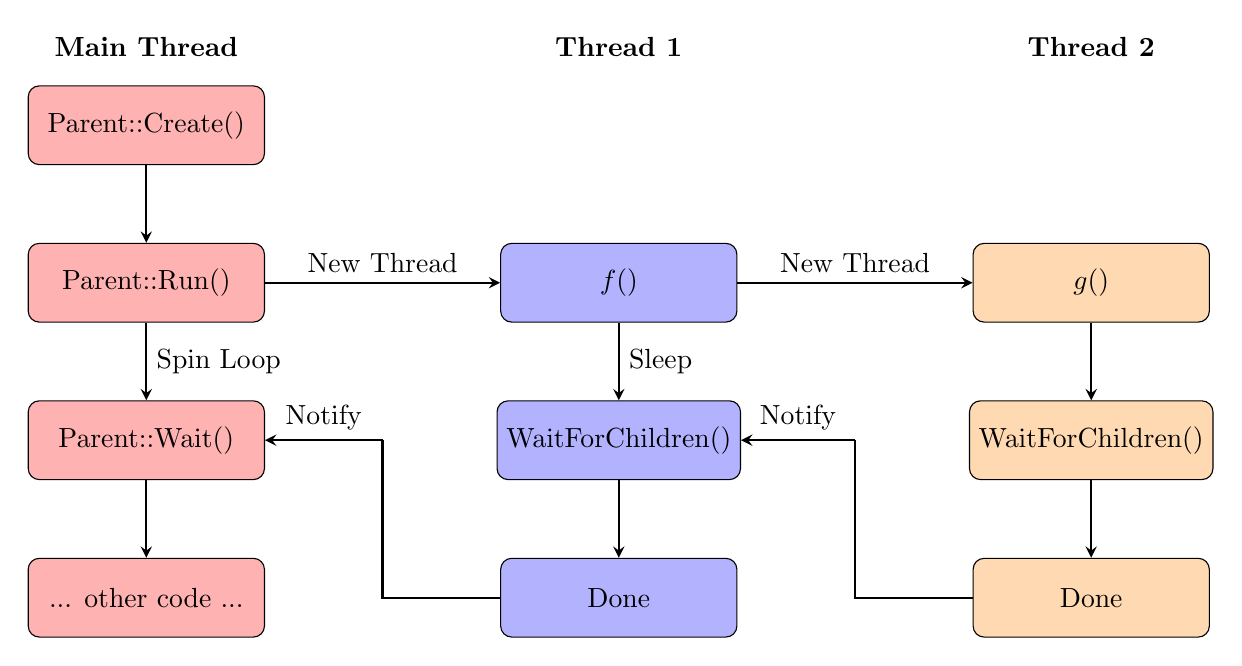
\begin{tikzpicture}[node distance=2cm]
                    % header nodes
                    \node (MainThread) {\textbf{Main Thread}};
                    \node (Thread1) [right of=MainThread, xshift=4cm] {\textbf{Thread 1}};
                    \node (Thread2) [right of=Thread1, xshift=4cm] {\textbf{Thread 2}};
                
                    % main thread nodes
                    \node (ParentCreate) [redrect, below of=MainThread, yshift=1cm] {Parent::Create()};
                    \node (ParentRun) [redrect, below of=ParentCreate] {Parent::Run()};
                    \node (ParentWait) [redrect, below of=ParentRun] {Parent::Wait()};
                    \node (ParentRest) [redrect, below of=ParentWait] {... other code ...};
                    
                    % thread 1 nodes
                    \node (Thread1Shim) [bluerect, right of=ParentRun, xshift=4cm] {$f$()};
                    \node (Thread1Wait) [bluerect, below of=Thread1Shim] {WaitForChildren()};
                    \node (Thread1Done) [bluerect, below of=Thread1Wait] {Done};
                    
                    % thread 2 nodes
                    \node (Thread2Shim) [orangerect, right of=Thread1Shim, xshift=4cm] {$g$()};
                    \node (Thread2Wait) [orangerect, below of=Thread2Shim] {WaitForChildren()};
                    \node (Thread2Done) [orangerect, below of=Thread2Wait] {Done};
                        
                    \node (Thread1WaitInvis) [right of=Thread1Wait, xshift=1cm] {};
                    \node (ParentWaitInvis) [right of=ParentWait, xshift=1cm] {};
                        
                    % arrows
                    \draw [arrow] (ParentCreate) -- (ParentRun);
                    \draw [arrow] (ParentRun) -- node [anchor=west] {Spin Loop} (ParentWait);
                    \draw [arrow] (ParentWait) -- (ParentRest);
                     
                    \draw [arrow] (ParentRun) -- node [anchor=south] {New Thread} (Thread1Shim);
                    \draw [arrow] (Thread1Shim) -- node [anchor=west] {Sleep} (Thread1Wait);
                    \draw [arrow] (Thread1Wait) -- (Thread1Done);
                    
                    \draw [arrow] (Thread1Shim) -- node [anchor=south] {New Thread} (Thread2Shim);
                    \draw [arrow] (Thread2Shim) -- (Thread2Wait);
                    \draw [arrow] (Thread2Wait) -- (Thread2Done);
                    \draw [thick] (Thread2Done) -| (Thread1WaitInvis.center);
                    \draw [arrow] (Thread1WaitInvis.center) -- node [anchor=south]{Notify} (Thread1Wait);
                    
                    \draw [thick] (Thread1Done) -| (ParentWaitInvis.center);
                    \draw [arrow] (ParentWaitInvis.center) -- node[anchor=south]{Notify} (ParentWait);
                \end{tikzpicture}
                
            
        \subsection{Creating Jobs Remotely}
            \subsubsection{Overview}    
                To issue jobs to different machines, MPI was used as the middleware to communicate with remote
                machines.This is superior to a custom-made server-client solution as MPI makes it easy to run programs
                on multiple machines.That being said, most MPI programs are run with a known number of nodes because
                it is specified as an argument via mpirun. However, for this library, we must spawn nodes dynamically
                as the user requests them. We define a \textit{master} node, who has the ability to spawn new children
                nodes who can be issued computational tasks. The master is also able to wait for the children to
                complete and query their status. 
                
                Once a child node has been spawned, there is no restriction on what it may run. It may run any CPU or
                GPU code, but may not spawn additional MPI children nodes, although nothing is stopping the programmer
                from directly accessing the MPI API. Custom packets were created using Google Protobuf to communicate
                commands, data, and notifications between the master and its children.
                 
            \subsubsection{Spawning New MPI Children Nodes}
                Spawning new MPI nodes dynamically is somewhat tricky. $\text{MPI\_Comm\_Spawn}$ will create a new
                node that can retrieve the parent's communicator, but each newly spawned set of nodes will have its
                own unique communicator. Because this library allows the user to spawn nodes one at a time, we must
                keep track of each child node's communicator. Furthermore, we must asynchronously probe each child
                communicator to check if any messages are waiting for us.
            
            \subsubsection{Issuing Commands to Children}
                
            
            \subsubsection{Children Synchronization and Termination}
        
            \subsubsection{TaskManager Class Reference}

    \section{Current Issues and Future Work}
    \section{Conclusion}
\end{document}
